

\tikzset{every picture/.style={line width=0.75pt}} %set default line width to 0.75pt        

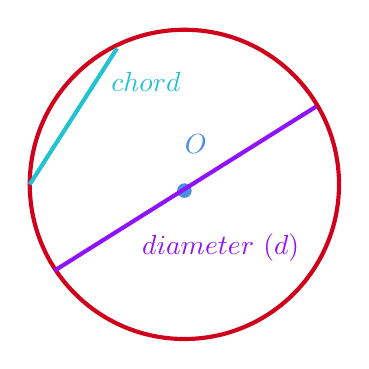
\begin{tikzpicture}[x=0.75pt,y=0.75pt,yscale=-1,xscale=1]
%uncomment if require: \path (0,188); %set diagram left start at 0, and has height of 188

%Shape: Circle [id:dp8118732481164563] 
\draw  [color={rgb, 255:red, 208; green, 2; blue, 27 }  ,draw opacity=1 ][line width=1.5]  (254,91.5) .. controls (254,50.35) and (287.35,17) .. (328.5,17) .. controls (369.65,17) and (403,50.35) .. (403,91.5) .. controls (403,132.65) and (369.65,166) .. (328.5,166) .. controls (287.35,166) and (254,132.65) .. (254,91.5) -- cycle ;
%Shape: Circle [id:dp14232976554180699] 
\draw  [color={rgb, 255:red, 74; green, 144; blue, 226 }  ,draw opacity=1 ][fill={rgb, 255:red, 74; green, 144; blue, 226 }  ,fill opacity=1 ] (325.83,93.13) .. controls (326.58,91.66) and (328.39,91.07) .. (329.87,91.83) .. controls (331.34,92.58) and (331.93,94.39) .. (331.17,95.87) .. controls (330.42,97.34) and (328.61,97.93) .. (327.13,97.17) .. controls (325.66,96.42) and (325.07,94.61) .. (325.83,93.13) -- cycle ;
%Straight Lines [id:da2079968527177969] 
\draw [color={rgb, 255:red, 144; green, 19; blue, 254 }  ,draw opacity=1 ][line width=1.5]    (266,133) -- (392,54) ;


%Straight Lines [id:da9513159212046638] 
\draw [color={rgb, 255:red, 33; green, 195; blue, 211 }  ,draw opacity=1 ][line width=1.5]    (296,26) -- (254,91.5) ;



% Text Node
\draw (334,72) node   {$\textcolor[rgb]{0.29,0.56,0.89}{O}$};
% Text Node
\draw (346,122) node   {$\textcolor[rgb]{0.56,0.07,1}{diameter\ ( d)}$};
% Text Node
\draw (310,42) node [color={rgb, 255:red, 33; green, 195; blue, 211 }  ,opacity=1 ]  {$\textcolor[rgb]{0.13,0.76,0.83}{chord}$};


\end{tikzpicture}